\chapter*{Introduction}
	Dans le cadre du module de \emph{Réseaux}, le projet de travaux pratiques portait sur la réalisation d'un protocole ou d'une application d'échange de données. Dans ce rapport, nous allons présenter les logiciels qui forment notre suite de messagerie instantanée que nous avons réalisé et qui permet l'échange de texte entre plusieurs clients via un serveur central. Ces programmes ont été réalisés dans le langage C comme précisé dans le sujet et utilisent les sockets bas niveau.
	
	Dans ce rapport, nous allons présenter dans un premier temps notre analyse du sujet et la manière dont nous avons pensé notre application. Ensuite, nous présenterons le fonctionnement de l'application en examinant les logiciels côté serveur puis client. 
		
\chapter{Analyse}
	\section{Présentation du sujet}
		Le sujet de ce projet portait sur la réalisation de programmes communiquants via le réseau via une architecture client / serveur.  Pour cela, nous devions utiliser le langage C, un des plus utilisé au monde et dont la caractéristique principale est d'être bas niveau, ce qui permet d'être un bon outil d'enseignement. En effet, cela permet de voir les briques de base d'un logiciel sans être pollué par une surcouche haut niveau.
		
		Pour nous aider, nous avons bénéficié d'un exemple étudié en TP et qui montrait les fonctions principales d'envoi et de reception de messages, ainsi que la manière d'utiliser les threads pour paralléliser les tâches d'un programme. Cela permet de pouvoir écouter et émettre en continu pour chaque connexion établie.

	\section{Choix du projet}
		À titre personnel, nous avions déjà réfléchi au développement d'un système de messagerie instantannée en peer-to-peer\footnote{Pair à pair : modèle de transmission où chaque noeud du système peut être client et serveur. Exemple : Bittorrent} (P2P) complètement décentralisé et sécurisé. Le but est qu'un utilisateur ne soit pas dépendant du bon fonctionnement d'un serveur central.\\
		
		Nous avons donc choisi pour ce TP de développer une application de messagerie instantannée type IRC\footnote{Internet Relay Chat} sur le modèle Client-Serveur, ce qui pourrait servir de base pour notre projet personnel.
		

	\section{Présentation des fonctionnalités}
		Nous nous sommes inspiré du protocole IRC, ce qui nous a permi d'identifier les fonctionnalités suivantes :
		\begin{itemize}
			\item Salon général de discussion : un utilisateur communique avec tous les autres qui sont connectés au même moment ;
			\item Messages privés : un utilisateur peut choisir de ne parler qu'à une personne à la fois sans que les autres ne puissent écouter ;
			\item Commandes d'utilisations : \verb!\quit! pour quitter, \verb!\help! pour obtenir une documentation légère, etc...
		\end{itemize}
		

\chapter{Fonctionnement du Chat}
	
	\section{Présentation du protocole}
		Parce qu'un schéma est plus parlant qu'un long discours, commençons par une présentation du protocole sous la forme d'un diagramme de séquence. Il est important de rappeler que comme toute architecture client/serveur, le client envoie des requêtes (ici sous la forme de messages) au serveur qui lui s'occupe d'agit en conséquence.
		\begin{figure}[h!]
			\centering
			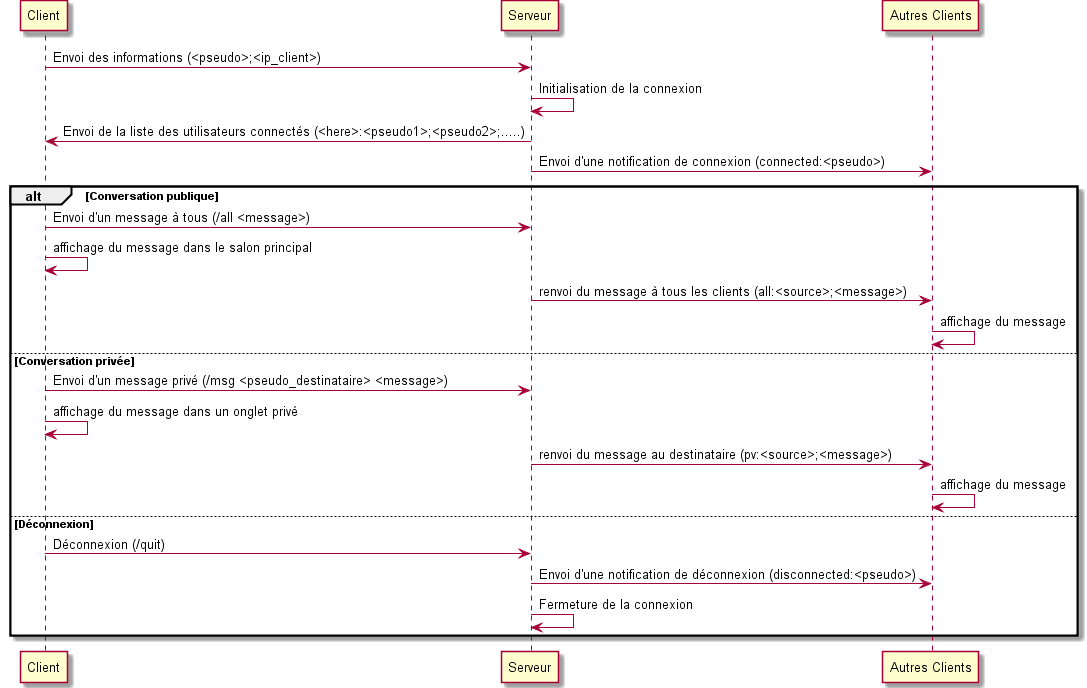
\includegraphics[scale=0.45]{protocol.png}
			\caption{Présentation générale du protocole utilisé.}
		\end{figure}
		\FloatBarrier
		
		L'entité \emph{Client} représente le client à partir duquel nous présentons notre protocole. C'est cette entité qui envoie les requêtes au serveur. Étant donné que le serveur est un intermédiaire entre plusieurs clients, nous avions besoin d'une autre entité. L'entité \emph{Autres Clients} représente donc les autres clients connectés au serveur, clients que nous n'étudions pas (un seul suffit à comprendre les spécifications du protocole) mais qui nous sert ici à montrer à quels moments les messages envoyés par \emph{Client} sont retransmis.\\
		
		Nous remarquons ici qu'une fois la connexion initialisée (le client et le serveur se connaissent et le serveur est prêt à écouter), le client n'a que trois possibilités :
		\begin{itemize}
			\item Engager une conversation dans le salon général ;
			\item Engager une conversation privée ;
			\item Se déconnecter.
		\end{itemize}
		
		Le protocole est donc très simple. Mais l'implémentation l'est moins du fait que le serveur doive pouvoir gérer plusieurs clients simultannément. Nous détaillerons donc le fonctionnement du serveur dans le chapitre suivant.
	
	\section{Fonctionnement du serveur}
		
		Côté serveur, il nous a paru évident qu'il faille implémenter une file de messages à envoyer de manière à ce que la réception de données ne soit pas bloquante. Pour utiliser cette file correctement, nous avons donc besoin de deux threads par client : un thread qui scrute la réception des requêtes du client et qui agit en conséquence, ainsi qu'un thread qui parcourt constamment la file de message afin de récupérer les messages à envoyer au client pour les retransmettre ensuite.
	
		\subsection{Liste des utilisateurs connectés}
			
			La liste des utilisateurs est un tableau de pointeurs vers des structures de données "utilisateurs" contenant deux chaînes de caractères : le pseudonyme (30 caractères maximum) et l'IP v4 (entre 7 et 15 caractères). Ce tableau est fixé en dur dans le code à 10 utilisateurs maximums simultanément pour ne pas surcharger le serveur dans le traitement des messages et des connexions/déconnexions.
			
			Lors de la demande de connexion d'un utilisateur, le serveur vérifie tout d'abord qu'il existe un emplacement libre pour un utilisateur supplémentaire (via une variable protégée par un mutex contenant le nombre de connexions en cours). Si la réponse est affirmative, les données de l'utilisateur sont ajoutées au tableau mais dans le cas contraire, l'utilisateur est informé de l'impossibilité de connexion et l'échange entre le client et le serveur s'arrête.
			
			Dans le cadre d'une déconnexion, le pointeur vers l'utilisateur dans la liste des connectés est mis à NULL et la structure est détruite. De plus, le nombre de personnes connectées est décrémenté pour faire de la place pour les suivants.
			
		\subsection{File de messages}
			La file de message est une structure C implémentée sous la forme d'une liste chainée. Chaque noeud contient plusieurs chaines de caractères décrivant le message à envoyer, l'expéditeur du message, ainsi que son destinataire.
			
			L'ajout d'un nouveau noeud s'effectue toujours à la fin de la file, de manière à pouvoir retourner le message le plus ancien le plus rapidement possible (envoyer le message le plus récent d'abord n'aurait pas de sens). Ainsi, la file est également dotée d'une fonction de défilage qui renvoie le premier message (donc le plus ancien) dont le destinataire correspond au thread qui demande un message pour son utilisateur.\\
			
			Cette file étant consultée et remplie par plusieurs threads à la fois, il est impératif de la protéger par un sémaphore d'exclusion mutuelle (mutex) qui la protège d'erreurs de pointeur (ajout dans la file alors qu'une opération sur les pointeurs est actuellement en cours, par exemple).
			
		\subsection{Thread de lecture}
			Un thread de lecture correspond à une communication avec un seul client, il y a donc autant de threads de lecture que d'utilisateurs. Lorsqu'une commande est envoyée au serveur, le serveur la traite et la transforme en un message avec une chaine de caractère de cette forme :
			\begin{itemize}
				\item \og pv;message \fg pour les messages publics;
				\item \og all;message \fg pour les messages privés;
				\item \og disconnected;pseudonyme \fg pour les déconnexions.
			\end{itemize}
			
			De cette manière, une chaîne de caractère correspond à une une action entre deux utilisateurs. Le message est ajoutée ensuite dans la liste avec le pseudo de l'expéditeur et du destinataire. Cependant, il est nécessaire de bloquer le sémaphore d'exclusion mutuelle pour ajouter afin d'éviter les écrasements de données ou autres conflits. 
			
			Dans le cas de la déconnexion ou du message public, il n'est pas nécessaire d'ajouter dans la liste la chaine autant de fois qu'il y a de destinataires différents : le destinataire sera "tout le monde", ce qui évite de remplir la liste trop rapidement. Les messages de connexions ne sont pas traités par ce thread mais sont aussi ajoutés à la liste de message.
			
		\subsection{Thread d'écriture}
			Un thread d'écriture a pour mission d'envoyer le message dans à la personne concernée. Pour cela, il lit en boucle le contenu de la file de message. Lorsqu'un message concerne l'utilisateur auquel il est lié, il l'enlève de la liste en bloquant le mutex puis le traite. Il en extrait le type d'information (publique, privée ou (dé)connexion), l'émetteur et le message.
			
			Il suffit ensuite de transmettre le message via le socket correspondant, le client fera ensuite le reste du traitement.
			
	
	\section{Fonctionnement du client}
		\subsection{Le coeur de l'application}
			Le client est constitué de trois fonctions principale.\\
			
			La première est celle de l'initialisation de la connexion. L'application demande des informations de connexion à l'utilisateur telles que le pseudo qu'il souhaite utiliser, son adresse IP (récupérée automatiquement mais dont on laisse la possibilité de modifier en cas d'erreur), ainsi que l'adresse IP et le port du serveur distant. Lorsque ces informations ont été récupérées, un paquet est forgé puis envoyé au serveur, qui va initialiser une connexion. Si quelque chose ne se passe pas correctement, l'application ferme en affichant un message d'erreur explicitant le problème.\\
			
			Dans le cas contraire, un FFFFRAIDE est créé. {\Huge TODO}\\
	
			\newpage
			Pour résumer, voici un schéma simplifié du fonctionnement des clients et du serveur lors de l'envoi de messages privés ou publics :
		
			\begin{figure}[h!]
				\centering
				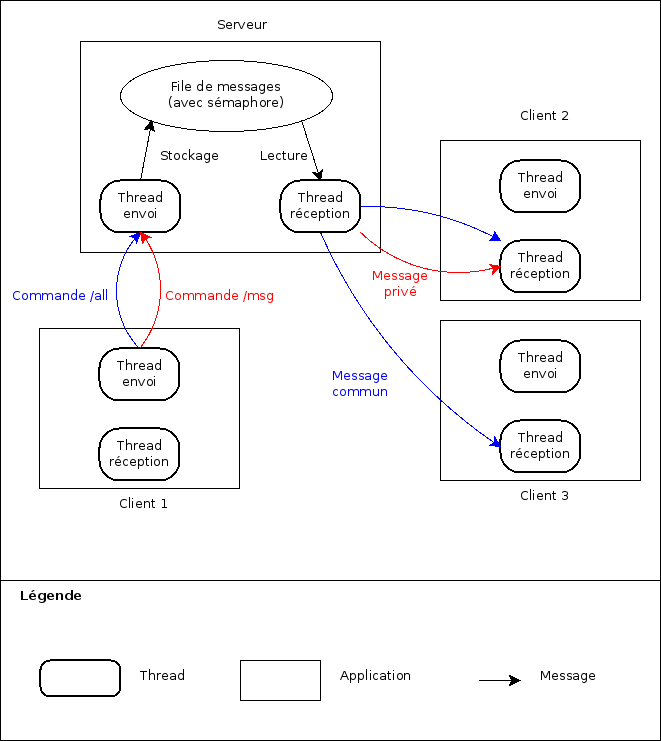
\includegraphics[scale=0.6]{echanges.png}
				\caption{Cheminement des messages lors de la communication inter-clients.}
			\end{figure}
			\FloatBarrier
		
			La dernière fonction est l'affichage de l'interface graphique, ainsi que la communication entre cette interface et le thread de communication avec le serveur. Nous détaillons cette fonction dans la partie suivante.
	
		\newpage
		\subsection{L'interface graphique}
			Étant donné que nous avons déjà utilisé Pidgin\footnote{Logiciel de messagerie} et l'avons trouvé \emph{user-friendly} et plutôt simple dans sa conception, nous nous en sommes inspirés.\\
			
			Nous avons utilisé le framework Qt.\\
			
			L'interface graphique est ainsi composée de quatres éléments principaux :
			\begin{itemize}
				\item Tout en haut, des onglets. À l'ouverture de l'application, seul l'onglet correspondant au salon principal est ouvert. Il permet ensuite de naviguer entre les différentes conversations privées ouvertes ;
				\item L'historique de conversation, qui domine la page ;
				\item À droite, la liste des utilisateurs actuellement connectés au salon. Pour entamer une conversation privée avec l'un d'entre eux, il suffit de faire un double clic sur celui qui nous intéresse ;
				\item En bas, un espace pour taper son message.
			\end{itemize}
			
			
			

\chapter*{Conclusion}
	Ce projet aura été l'occasion de consolider nos connaissances dans le domaine du réseau, et plus particulièrement dans le domaine des applications client/serveur. En effet, nous avons mis en place une architecture permettant à de multiples clients de partager des données (et plus particulièrement du texte) en passant par un serveur centralisé. Cela nous a permis de manipuler des sockets et des threads, éléments essentiels à tout informaticien lorsqu'il s'agit de faire des logiciels modernes : ils permettent l'interaction avec le réseau et la parallélisation des tâches.
	
	Parmi les évolutions envisageables, il sera possible dans une prochaine version de notre logiciel de s'affranchir du serveur centralisé pour réaliser une application répartie. Cela permettra de discuter sans dépendre d'une entité principale qui peut être surchargée ou indisponible, chaque client faisant aussi office de serveur. Notons aussi qu'il est possible de faire transiter par le réseau des fichiers pour permettre l'envoi de pièces jointes d'une machine à l'autre. Cette partie a été envisagée pendant le développement mais nous avons finalement décidé de nous concentrer sur les tâches les plus prioritaires et sur la correction de bogues.
